\documentclass[conference]{IEEEtran}
\IEEEoverridecommandlockouts
% The preceding line is only needed to identify funding in the first footnote. If that is unneeded, please comment it out.
\usepackage{cite}
\usepackage{amsmath,amssymb,amsfonts}
\usepackage{algorithmic}
\usepackage{graphicx}
\usepackage{textcomp}
\usepackage{multirow}
\usepackage{xcolor}
\usepackage{xspace}
\def\BibTeX{{\rm B\kern-.05em{\sc i\kern-.025em b}\kern-.08em
    T\kern-.1667em\lower.7ex\hbox{E}\kern-.125emX}}
\begin{document}

\newcommand{\etal}{{\it et al.}\xspace}
\newcommand{\eg}{{\it e.g.}\xspace}

\title{Configurable Hardware Accelerator of Misuse-Resistant Authenticated Encryption for Tightly-Constrained Environments}
\author{\IEEEauthorblockN{Mustafa~Khairallah}
\IEEEauthorblockA{\textit{School of Physical and Mathematical Sciences} \\
\textit{Nanyang Technological University}\\
Singapore, Singapore \\
mustafa.khairallah@ntu.edu.sg
}
}

\maketitle

\begin{abstract}
Nonce-misuse is a frequently overlooked threat in tightly-constrained environments, either because of a gap of understanding, or the high cost of solutions to such problem. Among the candidates for NIST lightweight cryptography standardization, only one includes a nonce-misuse-resistant variant for confidentiality and integrity; Romulus-M, and its performance is almost not studied in practice. In this paper, we study the performance of this scheme in comparison to other AEAD schemes, especially its non-misuse-resistant variant; Romulus-N. We provide a family of configurable accelerators for both Romulus-N and Romulus-M, showing that the cost of adding Romulus-M with Romulus-N in the same implementations is very small in terms of area. We show that Romulus-M is less than 50\% slower than Romulus-N for short messages, and less than 65\% slower for long messages, for low-area iterative configurations. We study the performance compared to AES-GCM, the defacto AEAD algorithm in practice, and other lightweight cryptography standardization candidates. We also provide the first hardware implementations of Romulus compatible with both Tweakable Block Ciphers (TBCs) in the ISO/IEC NP 18033-7 standard proposal, with support for both Skinny and Deoxys-BC TBCs. The compile-time configurations of our accelerator include choosing the TBC, the latency of the TBC, bus width and the number of plaintext and key shares. During runtime, the user can select between Romulus-N and Romulus-M using input instructions. The results show that Romulus-M is a competitive candidate in its own regard, not just as an extra layer of protection on top Romulus-N.
\end{abstract}

\begin{IEEEkeywords}
Authenticated Encryption, Tweakable Block Ciphers, Accelerators, Lightweight Cryptography, Romulus, Integrity, Privacy
\end{IEEEkeywords}

\section{Introduction}

Lightweight cryptography is the field of cryptology that studies cryptographic schemes targeted at achieving competitive performance at low cost. Specifically, it targets environments where classical symmetric-key encryption algorithms, such as the Advanced Encryption Standard (AES)~\cite{daemen2001reijndael} and the AES-GCM Authenticated Encryption with Associated Data (AEAD) mode~\cite{mcgrew2004galois}, are either infeasible or too costly. An AEAD mode is a symmetric-key cryptographic scheme designed to offer both integrity and confidentiality, simultaneously. It takes three inputs: plaintext $M$, secret key $K$ and public associated data $A$, and outputs a ciphertext $C$ and an authenticated tag $T$. In 2019, the National Institute for Standardization and Technology (NIST), USA, accepted 56 AEAD candidates for standardization~\cite{turan2019status}, and narrowed them down to 10 finalists in 2021~\cite{turan2021status}. Each submission includes one main variant, and optionally other variants that offer extra features. All the main partially derive their security from an extra public input known as either {\it nonce} ($N$) or {\it Initial vector} ($IV$), where for a given secret key $K$, $N$ must be unique for every message and must not be repeated. While this leads to the design of fast and cheap AEAD scheme, it leads to implementation problems, as the either the implementation, the higher-level communication protocol or the user must ensure that the nonce is never repeated. This requires additional storage and implementation mechanisms not accounted for in the AEAD cost. Besides, the ambiguity about the responsibility of generating the nonce has been identified by researchers as a security threat. In 2022, Shakevsky \etal~\cite{shakevsky2022trust} have shown that Samsung flagship smartphones, including S21, use AES-GCM as an AEAD scheme and are vulnerable to nonce-misuse attacks.

On the flip side, AEAD schemes that are not vulnerable to nonce-misuse attacks, and can be implemented even without any nonce or with a fixed nonce have been proposed by researchers. In their seminal work~\cite{rogaway2006provable}, Rogaway and Shrimpton proposed the Synthetic-IV (SIV) scheme, which was followed up by other misuse-resistant schemes (\cite{jean2016deoxys,gueron2017aes}). However, these schemes require the input to be processed twice, which is a limitation that cannot avoided to achieve nonce-misuse.

In the context of the NIST lightweight cryptography standardization project, only Romulus~\cite{iwataromulus} includes a variant; Romulus-M, that offers integrity and confidentiality against nonce-misuse adversaries, while Elephant~\cite{dobraunig2019elephant} only offers integrity against nonce-misuse adversaries, without privacy. However, the hardware performance of Romulus-M has been under-studied.

\paragraph{Contributions.} In this paper, the design of a configurable hardware accelerator for the Romulus AEAD family is proposed. The design simultaneously supports the nonce-respecting variant Romulus-N and the misuse-resistant variant Romulus-M. Besides, it can be configured to support the newly proposed ISO standard: ISO/IEC 18033-7 for Tweakable Block Ciphers~\cite{iso}. We show that Romulus-M can be implemented with almost zero-overhead in terms of area, compared to Romulus-N and less than 60\% slow-down.

Comparative studies of new standardization proposals, such as this one, help understand the performance of new designs and inform standards' authors and implementation designers alike. Particularly, understanding the performance of the misuse-resistant AEAD scheme Romulus-M is needed as part of the NIST standardization efforts.

\section{Background}

\subsection{Nonces}

The security of SKE is dependent, by definition, on the secrecy of a shared secret key $K$ between communicating parties. In practice, however, the security of many SKE schemes, including most AEAD schemes, relies also on the properties of another parameter that is usually public, and is referred to as a Nonce $N$ or an Initial vector $IV$. This public parameter is usually assumed to be unique and cannot be repeated for two different messages (nonce-based AEAD) or uniformly random ($IV$-based AEAD).

Both of the aforementioned requirements are hard to enforce in practice. They rely on a threat model that assumes the user and implementer are both honest and understand the security requirements. To the contrary, it was shown that these assumptions may not hold even in widely-used commercial products, designed with the promise of hardware security. In February 2022, Shakevsky \etal showed an $IV$-reuse attack on the AES-GCM encryption algorithm on a range of flagship Android-powered Samsung smartphones~\cite{shakevsky2022trust}.

Such attacks necessitate more careful handling of nonces. This can be done in one of two ways.

\begin{enumerate}

\item Ensure the implementations use nonces that satisfy the assumptions that the AEAD scheme is based on, \eg uniqueness. However, this approach is what is being assumed currently. This leads either complicated and costly implementations, or implementation mistakes that can leads to cryptographic breaks.
\item Rely on AEAD schemes that are more robust to nonce repetition or non-randomness. On the bright side, this issue have been studied by cryptographers, schemes such as SIV~\cite{rogaway2006provable}, AES-GCM-SIV~\cite{gueron2017aes}, Deoxys-II~\cite{jean2016deoxys} and, more recently, Romulus-M.
\end{enumerate}

\begin{figure}[!t]
  \centering
  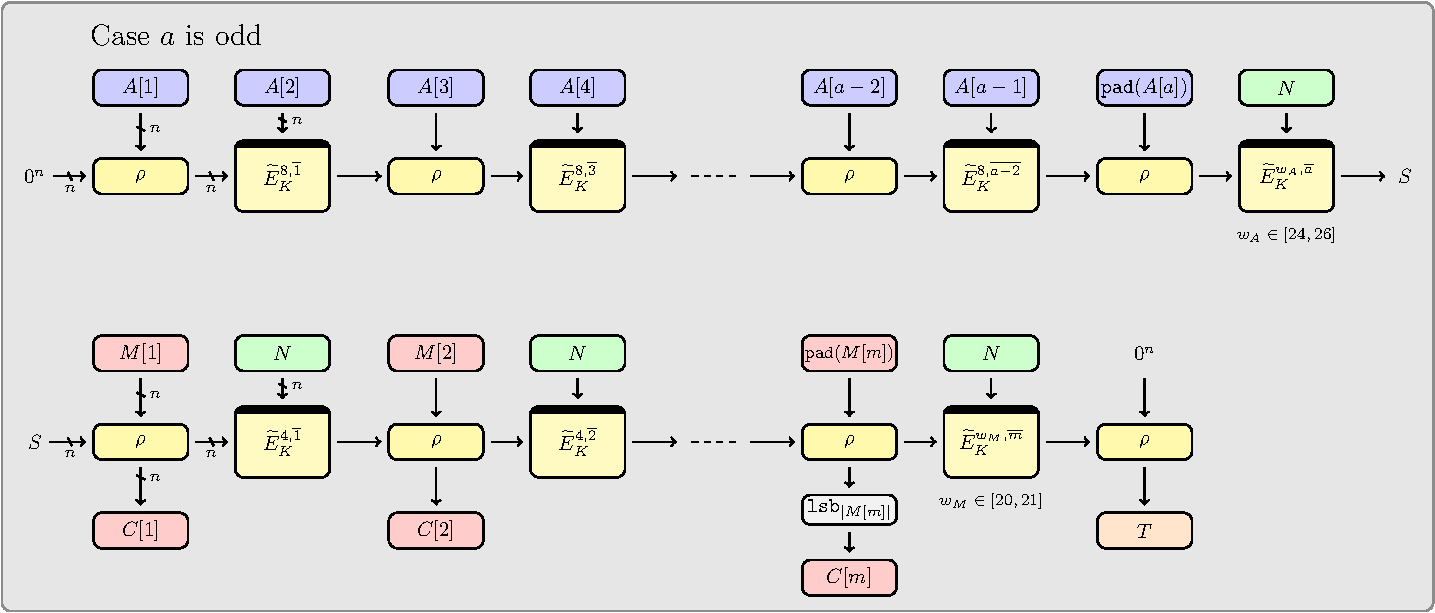
\includegraphics[width=0.49\textwidth]{figures/mode_simplified.pdf}
  \caption{The Romulus-N AEAD scheme~\cite{romulus_site}.}\label{fig:romulusn}
\end{figure}

\subsection{Romulus}

Romulus~\cite{iwataromulus} is a finalist in the NIST lightweight cryptography standardization project. It is based on the SKINNY TBC~\cite{beierle2016skinny} and incurs very small overhead in terms of storage compared to the underlying TBC. The schemes presented, however, are independent of the underlying TBC~\cite{iwata2020duel}. In this paper, we focus on two variants of the Romulus family:

\begin{enumerate}
\item {\it Romulus-N} is a nonce-respecting AEAD scheme, depicted in Figure~\ref{fig:romulusn}.
\item {\it Romulus-M} is a misuse-resistant AEAD scheme, depicted in Figure~\ref{fig:romulusm}. Additionally, it offers security even if unauthenticated plaintext is released during decryption, which is a security model targeted for hardware accelerators with small memory~\cite{andreeva2014securely}.
\end{enumerate}

Romulus-N is the main variant of the Romulus family, and almost all of the analysis and benchmarking have been done on this variant. However, Romulus-N fails under the security threats of nonce-reuse and Release of Unverified Plaintext (RUP). Romulus-M, on the other hand, ensures security even in the presence of nonce-misuse and RUP.

\begin{figure*}[!t]
  \centering
  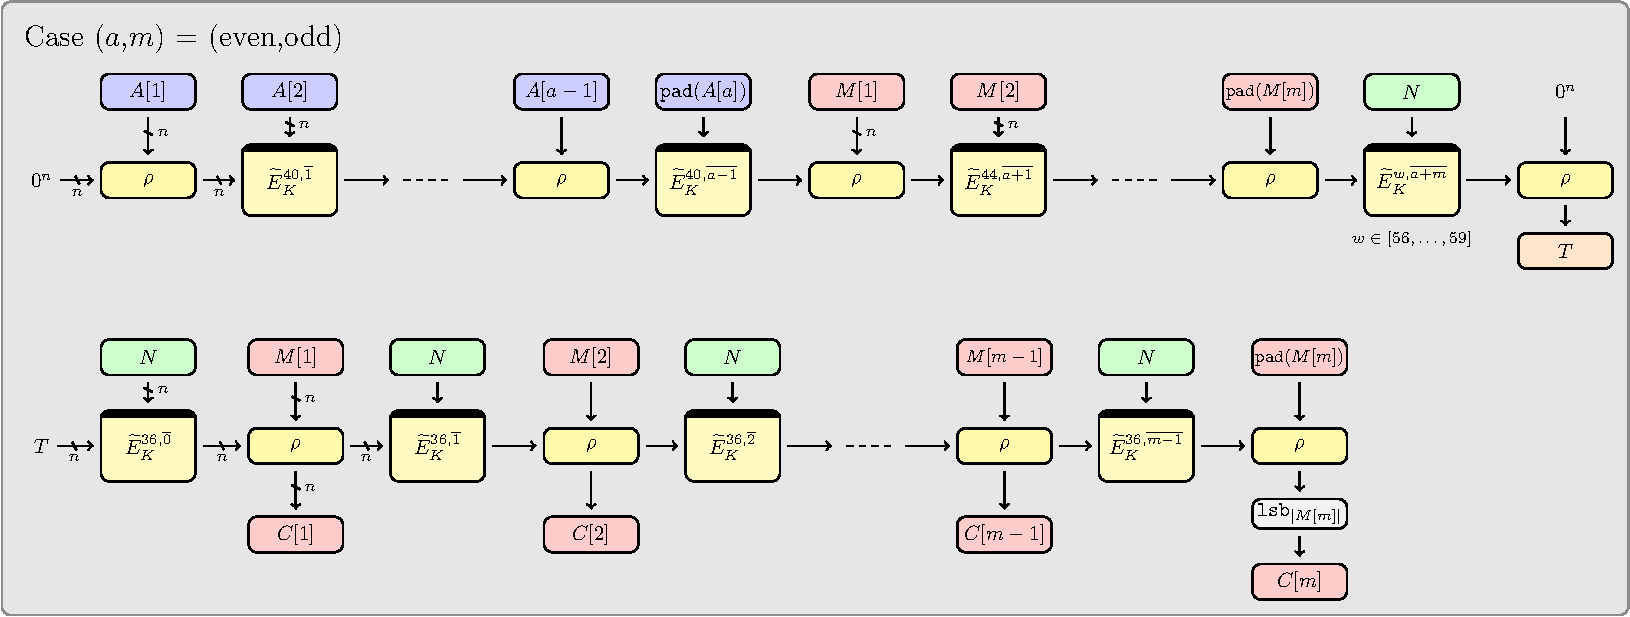
\includegraphics[width=0.7\textwidth]{figures/modeM_simplified.pdf}
  \caption{The Romulus-M AEAD scheme~\cite{romulus_site}.}\label{fig:romulusm}
\end{figure*}

\subsection{Tweakable Block Ciphers}

A TBC is a keyed function $\tilde{E}$ that takes three inputs: a secret key $K$, a public tweak $T$ and an $n$-bit message block $M$. For each selection of $(K,T)$, it behaves as a random permutation over the space of $n$-bit binary strings. A TBC is superior to a classical BC due to the extra public tweak $T$. TBCs have been formalized in~\cite{liskov2002tweakable} and have been a useful tool in the field of SKE encryption and design for years. Since the introduction of the $\Theta$CB-3~\cite{krovetz2011software} and the design of the Deoxys-BC~\cite{jean2016deoxys}, more and more research have been performed in order to design practical, efficient and cheap TBCs and TBC-based schemes. Recently, two TBCs have been considered for the final stages of ISO standardization; Deoxys-BC and SKINNY. Deoxys-BC is the basis of Deoxys, the winner of the CAESAR competition for AEAD designs. SKINNY, on the other hand, is the basis for Romulus, a finalist in the NIST lightweight cryptography standardization project.

\subsection{Implementations}

The implementations explored in this paper are built using the Verilog HDL language, and studied using the iVerilog~\cite{iverilog} and VCS simulators and the Synopsys Design Compiler synthesizer. The technology targeted is TSMC 65nm. The implementations will be made available as open source with the final version of this paper.

\section{ISO/IEC 18033-7: Deoxys-BC and SKINNY}\label{sec:tbc}

The ISO/IEC 18033-7 is currently in the {\it ``under-development''} stage. It specifies the two TBCs: SKINNY and Deoxys-BC. In this section, we look at there combinational cost of there largest variants, with block size of 128 and tweakey size of 384. We assume they are used either as CPU co-processor or inside an iterative hardware accelerator that operates on the full 512-bit state in a single clock cycle. Hence, the smallest implementation is the round-based implementation; the combinational circuit performs 1 round per call/clock cycle. Deoxys-BC and SKINNY share similar design principles and they are both based on the tweakey framework. They are both based on the STK framework~\cite{jean2014tweaks} and Substitution-Permutation Networks (SPNs). Each round consists of 4 operations: SBoxLayer, AddRoundTweakey, ShiftRows, and MixColumn, with slightly different order. Deoxys-BC has an extra AddRoundTweakey operation in the final round. SKINNY-128-384+ consists of 40 rounds, while Deoxys-BC-128-384 consists of 16 rounds. However, since the internal components are different, SKINNY's round function is a lot smaller than that of Deoxys-BC. A common misconception is a cipher with less rounds is faster than a cipher with more rounds. This is not true, as the definition of a round is arbitrary and our experiments show that SKINNY can be faster than Deoxys-BC in many use-cases. While SKINNY is targeted towards lightweight and low-area applications, our experiments show that Deoxys-BC is only faster than SKINNY at very high frequencies, and this comes at a huge area cost. Besides, such high frequencies maybe unachievable. The cipher will be used inside a processor or a hardware accelerator, and the frequency will be decided by other parts of the system; {\it e.g.} CPU, Finite State Machine (FSM)...{\it etc.}

We assume that all calls have the same number of rounds, such the combinational circuit of SKINNY can perform 1, 2, 4, 5, 8, 10, 20 or 40 rounds, while the circuit of Deoxys-BC can perform 1, 2, 4, 8, or 16 rounds. Since Deoxys-BC uses the AES round function, we considered two possible configurations for the SBox: Look-Up Table (LUT), which is more suitable for high-speed and FPGA implementations, as discussed in~\cite{khairallah2017looting}, and a low-area SBox circuit~\cite{boyarperlata,tinyaes}, which suitable for low-area ASIC implementations. Table~\ref{tab:comptbc} shows the synthesis results for these configurations on the TSMC 65nm standard cell library. While the speed of a hardware accelerator or an SoC is not determined just by the cryptographic combinational circuit, this section can be viewed as investigating the limits of these TBCs. For example, Table~\ref{tab:comptbc} shows that the circuit cannot be computed on the considered technology in with less than 17.4ns, while Deoxys-BC cannot computed in less than 12.91ns. When we add a 0.5ns safety slack per call, these numbers grow to 19.97ns and 13.4, respectively. However, when we also compare the area, we see that the faster implementation of Deoxys-BC comes at a huge area cost, where the fastest implementation of SKINNY costs 2228.75 and 52892.5, respectively, while for Deoxys-BC, the best latency is achieved at 174169.24 GE. SKINNY also has the potential to be 7 times more efficient than Deoxys-BC at high frequencies, and 2.3 times more efficient at 24 MHz. At low frequencies, the efficiency of both TBCs becomes almost constant, in which case they both offer an interesting straight-forward trade-off between speed and area. Note that these values are only for the combinational part of the cipher, and the efficiencies will drop when the storage is added. However, we exclude the storage from this section as the storage should be part of the higher-level system. In the next section, we will revisit how SKINNY and Deoxys-BC can be used inside existing systems without requiring any extra storage.

\begin{table*}[!thb]
\centering
\caption{Comparison of the logic circuit of Skinny and Deoxys-BC for different value of latency. Synthesis results are using TSMC 65nm.}\label{tab:comptbc}
\begin{tabular}{c|c|c|c|c|c|c|c|c}\hline
  \multirow{2}{*}{\textbf{TBC}} & \multirow{2}{*}{\textbf{\# of Rnds}} & \multirow{2}{*}{\textbf{\# of Cycles}} & \textbf{Area} & \textbf{Critical Path} & \textbf{Min. Latency} & \textbf{Safe Latency} & \textbf{$\frac{128000}{L\times A}$}  & \multirow{2}{*}{\textbf{$\frac{128000}{L\times A}$ at 24MHz}} \\
  & & & \textbf{(GE)} & \textbf{(ns)} & \textbf{(ns)} & \textbf{(ns)} & \textbf{at min. latency.} & \\ \hline \hline
  \multirow{8}{*}{Skinny} &
    1	& 40 & 1107 & 0.44	& 17.6	& 37.6 & 6.57 & 0.07 \\
  & 2	& 20 & 2228.75 & 0.87	& 17.4	& 27.4 & 3.3 & 0.07 \\
  & 4	& 10 & 4790.5 & 1.94	& 19.4	& 24.4 & 1.37 & 0.06 \\ 
  & 5	&  8 & 6029.5 & 2.56	& 20.48	& 24.48 & 1.03 & 0.06 \\
  & 8	&  5 & 10117 & 3.86	& 19.3	& 21.8 & 0.66 & 0.06 \\
  & 10 & 4 & 12776.75 & 4.94	& 19.76	& 21.76 & 0.51 & 0.06 \\
  & 20 & 2 & 26554.68 & 9.78	& 19.56	& 20.56 & 0.25 & 0.06 \\
  & 40 & 1 & 52892.5 & 19.47 & 19.47 & 19.97 & 0.12 & 0.06 \\
    \hline
    \multirow{5}{*}{Deoxys-BC LUT} &
    1 & 16 & 9825.25& 0.88 & 14.08 & 22.08 & 0.93 & 0.02 \\
    & 2 & 8 & 20998& 1.7 & 13.6 & 17.6 & 0.45 & 0.02 \\
    & 4 & 4 & 43588.5& 3.4 & 13.6 & 15.6 & 0.22 & 0.02 \\
    & 8 & 2 & 86156.25& 6.65 & 13.3 & 14.3 & 0.11 & 0.02 \\
    & 16 & 1 & 174169.24& 12.91 & 12.91 & 13.4 & 0.06 & 0.02 \\
    \hline
    \multirow{5}{*}{Deoxys-BC BP} &
    1 & 16 & 7347.25& 1.26 & 20.16 & 28.16 & 0.86 & 0.03 \\
    & 2 & 8 & 19346 & 2.39 & 19.12 & 23.12 & 0.35 & 0.02 \\
    & 4 & 4 & 43634 & 4.43 & 17.72 & 19.72 & 0.17 & 0.02 \\
    & 8 & 2 & 91086.11& 8.78 & 17.56 & 18.56 & 0.08 & 0.02 \\
    & 16 & 1 & 181776 &  16.71 &  16.71 &  17.21 &  0.04 & 0.02 \\ \hline
\end{tabular}
\end{table*}



\section{Romulus-N/M Hardware Accelerator}

The proposed architecture compliant with the lightweight cryptography hardware API proposed in~\cite{kaps2019hardware}. This choice is to allow fair comparison to other implementations and to allow a full implementation that does not ignore any hidden costs such as key storage, nonce storage or message padding. The architecture is parameterized by the following parameters:
%
\begin{itemize}
\item $w$: bus width, defaulted to 32 bits.
\item $S_s$: number of state shares; used for masked implementations, defaulted to 1.
\item $K_s$: number of secret key shares; used for masked implementations, defaulted to 1.
\item $TBC$: choice of the TBC.
\item $r$: number of TBC rounds per cycle.
\end{itemize}
%
The architecture, depicted in~\ref{fig:arch}, is built based on 4 register files:
%
\begin{enumerate}
\item State Register File (SRF): consists of $128\times S_s/w$ words, each consists of $w$ bits.
\item Key Register File (KRF): consists of $128\times K_s/w$ words, each consists of $w$ bits.
\item Tweak Register File (TRF): consists of $128/w$ words, each consists of $w$ bits. Since the tweak is always public, it does not need to be masked.
\item Counter Register File (CRF): consists of $128/w$ bits.
\end{enumerate}

The SRF is reset to 0 at the beginning a new encryption or decryption instruction. It is loaded in the feedback mode, where the $G$ function is applied to the bottom word in a byte-wise fashion. It transforms each byte as follows:
\[
(x_0,x_1,x_2,x_3,x_4,x_5,x_6,x_7)\rightarrow
\]
\[
(x_1,x_2,x_3,x_4,x_5,x_6,x_7,x_0\oplus x_7)
\]
%
The output of this transformation is XORed with the input word (from the control unit) to generate the plaintext during encryption and the ciphertext during decryption. The plaintext (the input word during authentication and encryption, and the output of the previous XOR during decryption) is XORed with bottom word to generate the feedback word that get fed from the top, shift all the other words down. In order to support Romulus-M, a bypass connection is needed such that the tag from the top operation in Figure~\ref{fig:romulusm} is fed back into the SRF. This bypass connection is shown in red in Figure~\ref{fig:arch}. The KRF and TRF are similar, where they are loaded from the top down, with no feedback needed. The CRF is used to hold the block counter and the domain separator; the constant part of the public tweak. It does not need a load operation, as it is reset to the initial value of the counter. Each register file can also be read and written in parallel, where the circuit from Section~\ref{sec:tbc} is represented in Figure~\ref{fig:arch} by the combination of TBC, Key Schedule, Tweak Schedule and Domain Separator Schedule.

During execution, the nonce will be stored in the TRF, while the secret key will be stored in the KRF. There values will be changed, and needs to be corrected during, which the purpose of the Secret Key Correction and Tweak Correction circuits. These operations, alongside the Counter, are performed in between the TBC calls, in parallel to loading the SRF.
%
\begin{figure*}[!htb]
  \centering
  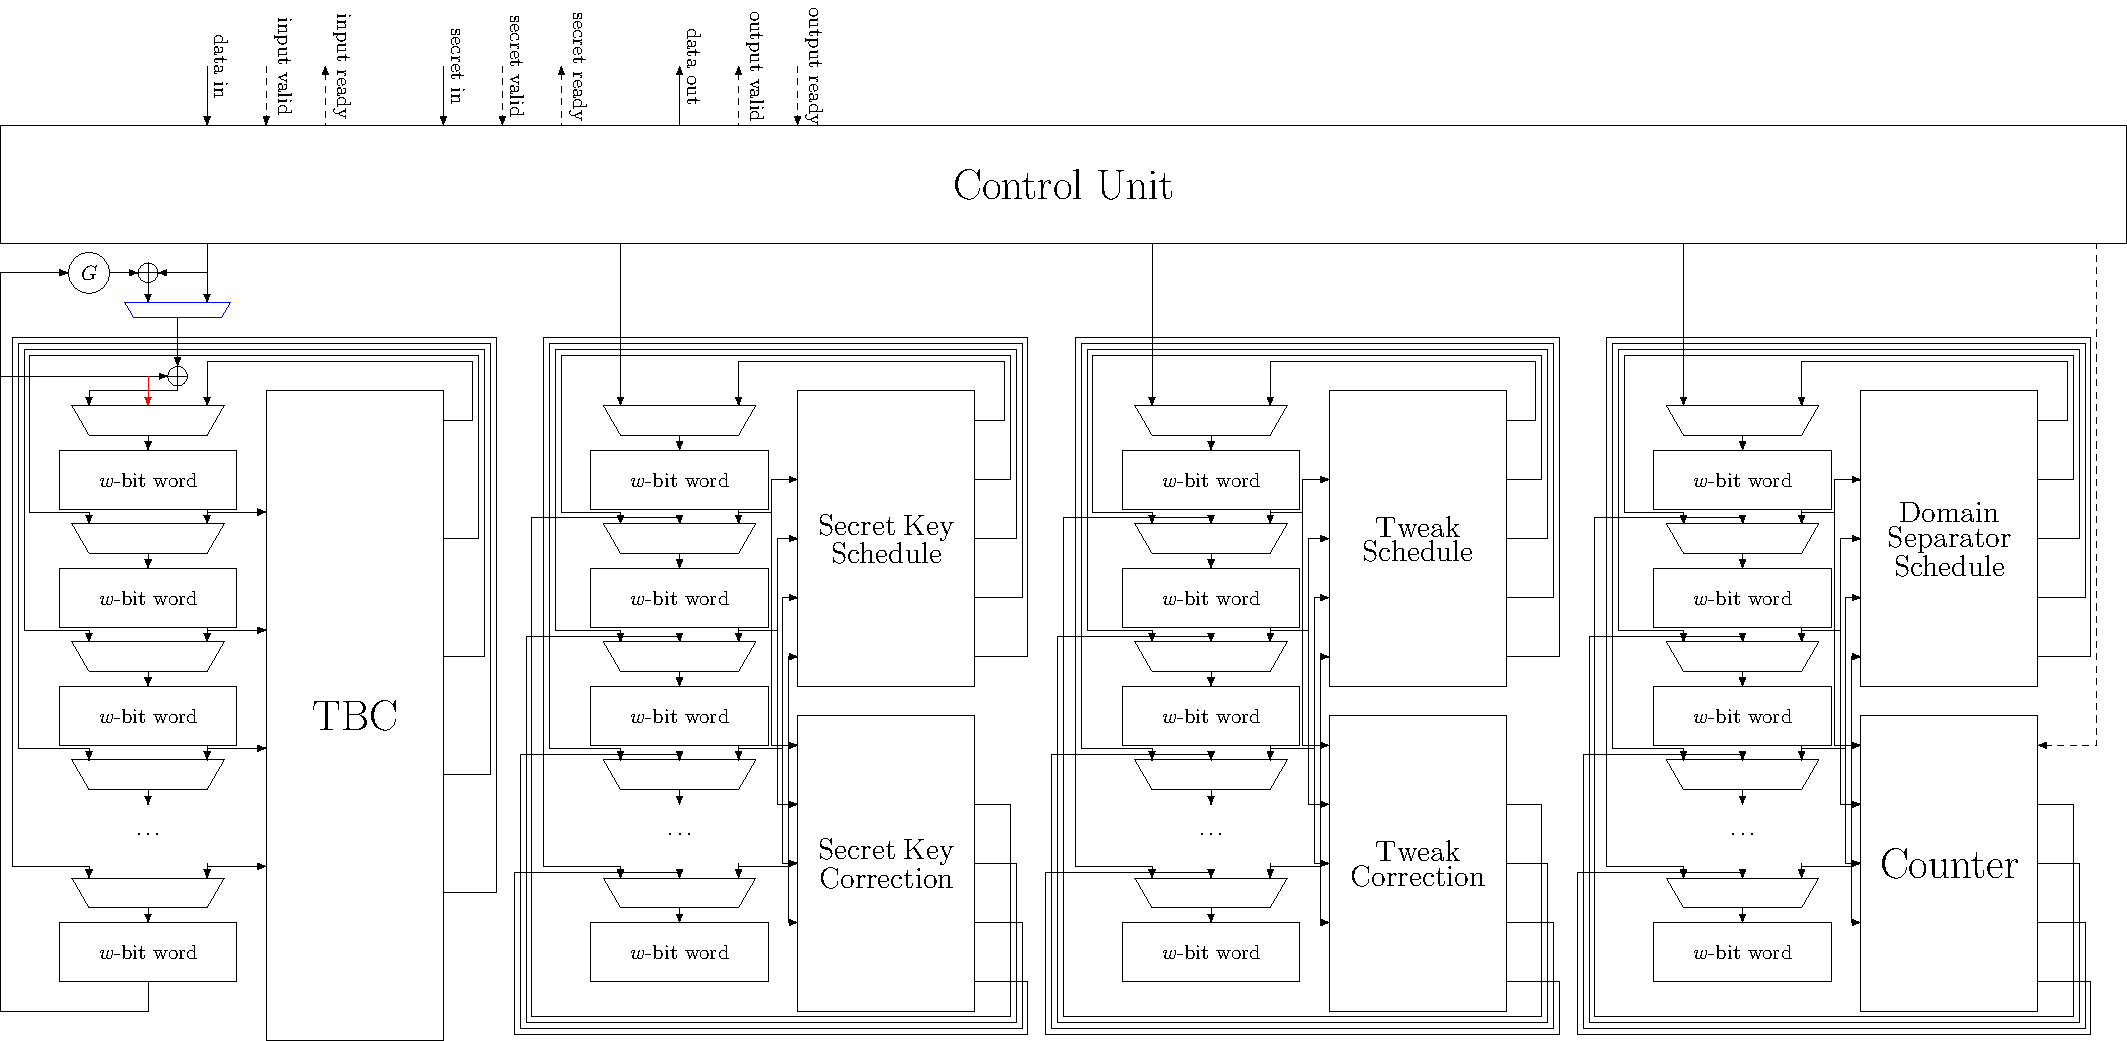
\includegraphics[width=\textwidth]{arch_diagram.pdf}
  \caption{The architecture of the proposed hardware accelerator. Solid arrows are $w$-bit wide, where $w$ is the configurable bus width. The dotted arrows are control signals. Some of the control signals are omitted from the diagram for simplicity including multiplexers' selectors, registers enables and resets. The red arrow is only needed for Romulus-M and can be removed if Romulus-M support is not required. The blue multiplexer is used to switch between encryption and decryption.}\label{fig:arch}
\end{figure*}

Table~\ref{tab:instlatency} shows the latencies of the proposed architecture for both Romulus-N and Romulus-M encryption instructions, for different sizes on $A$ and $M$, where $a$ and $m$ are the number of bytes of $A$ and $M$, respectively. This is shown when $w=32$, and both the state and key are unmasked. The latencies do not depend on the TBC used. The bottom section of Table~\ref{tab:instlatency} includes the ratio between the latency of Romulus-M and Romulus-N, where for short messages (64 bytes of $A$ and $M$) and low area (high latency), the ratio is about 1.3, while for longer message low area configurations the ration is less than 1.4. For empty $A$, the ratio is less than 1.65 for low area configurations.

\begin{table}[!thb]
  \centering
  \caption{Latency of Romulus-N and Romulus-M for different latencies of the TBC. $w=32$}\label{tab:instlatency}
  \begin{tabular}{c|c|c|c|c|c|c|c}\hline
  \textbf{Mode} & \textbf{$a$} & \textbf{$m$} & 40 & 20 & 10 & 4 & 1 \\\hline \hline
  \multirow{7}{*}{N} & 0 & 0 & 101 & 61 & 41 & 29 & 23 \\
  &  0 & 64 & 237 & 137 & 87 & 57 & 42 \\
  & 64 &  0 & 197 & 117 & 77 & 53 & 41 \\ 
  & 64 & 64 & 333 & 193 & 123 & 81 & 60 \\
  & 0 & 1152 & 3225	& 1765	& 1035	& 597	& 378 \\
  & 1152 & 0 & 1825	& 1065 &	685	& 457	& 343 \\
  & 1152 & 1152 & 4949 & 2769 & 1679	& 1025 & 698 \\ \hline

  \multirow{7}{*}{M} & 0 & 0 & 101	& 61	& 41	& 29	& 23 \\
  &  0 & 64 & 338	&198	&128	&86	&65 \\
  & 64 &  0 & 157	& 97	&67	&49	&40  \\ 
  & 64 & 64 & 434	&254	&164	&110	&83 \\
  & 0 & 1152 & 4954	&2774	&1684	&1030	&703 \\
  & 1152 & 0 & 1785	&1045	&675	&453	&342 \\
  & 1152 & 1152 & 6678	&3778	&2328	&1458	&1023 \\ \hline

  & 0 & 0 & 1.00	& 1.00	& 1.00	& 1.00	& 1.00 \\
  Latency& 0& 64& 1.43	& 1.45	& 1.47	& 1.51	& 1.55 \\
  Overhead& 64& 0& 0.79	& 0.83	& 0.87	& 0.92	& 0.98 \\
  & 64& 64& 1.30	& 1.32	& 1.33	& 1.36	& 1.38 \\
  & 0& 1152& 1.57	& 1.57	& 1.63  & 1.72	& 1.86 \\
  & 1152& 0& 0.99	& 0.98	& 0.98	& 0.99	& 1.00 \\
  & 1152& 1152& 1.35	& 1.36	& 1.39	& 1.42	& 1.47 \\ \hline
  \end{tabular}
\end{table}

Table~\ref{tab:acc65nm} shows the synthesis results for a group of unmasked configurations for both SKINNY and Deoxys-BC, for both maximum frequency and low area 24 MHz constraints. Our experiment shows that with SKINNY, both Romulus-N and Romulus-M achieve the minimum energy consumption when the TBC latency is 10 cycles (4 rounds per cycle), while with Deoxys-BC the minimum energy is achieved when the TBC latency is 16 (one round per cycle). Low latency implementation (1 clock cycle per TBC) can be achieved using SKINNY (40 rounds) in around 55 kGE. Besides, for around the same area ($\approx 12$ kGE), Romulus with SKINNY is 1.85 and 1.7 times fast than Romulus with Deoxys-BC for N and M, respectively. For high frequencies, Romulus with Deoxys-BC is 1.24 and 1.34 faster for N and M, respectively. At 24MHz, the single-cycle implementation of SKINNY can achieve relatively high speeds.

\begin{table*}
  \centering
  \caption{Synthesis result of the proposed hardware accelerator on TSMC 65nm.}\label{tab:acc65nm}
  \begin{tabular}{c|c|c|c|c|c|c|c|c|c|c|c|c|c}\hline
    \multicolumn{2}{c|}{}&\multicolumn{6}{c|}{\textbf{24MHz}}&\multicolumn{6}{c}{\textbf{High Speed}} \\ \hline
    \textbf{TBC} & \textbf{Area} & \textbf{CP} & \textbf{Power} & \textbf{Th/put} &  \textbf{Th/put} & \textbf{Energy} & \textbf{Energy} & \textbf{CP} & \textbf{Power} & \textbf{Th/put} &  \textbf{Th/put} & \textbf{Energy} & \textbf{Energy}  \\ 
    \textbf{Rounds} & \textbf{(GE)} & \textbf{(ns)} & \textbf{(mW)} & \textbf{(Mbps)} & \textbf{(Mbps)} & \textbf{(pJ/bit)} &  \textbf{(pJ/bit)}  & \textbf{(ns)}& \textbf{(mW)} & \textbf{(Gbps)} & \textbf{(Gbps)} & \textbf{(pJ/bit)} &  \textbf{(pJ/bit)}   \\
    & & &  & \textbf{N} & \textbf{M} &\textbf{N} & \textbf{M}  && & \textbf{N} & \textbf{M} & \textbf{N} & \textbf{M}  \\ \hline \hline
    \multicolumn{11}{c}{SKINNY} \\ \hline
    1  & 7348.61   & 1.11	  & 0.22    &  89 &  66 & 2.47	& 3.33 & 1.5 & 0.74 & 2.48 & 1.84 & 0.30 & 0.40 \\ 
    2	 & 7865.28	 & 1.16		& 0.24		& 159 & 117 & 1.49  & 2.04 & 1.5 & 0.74 & 2.43 & 3.25 & 0.17 & 0.23 \\ 
		4	 & 10124.24	 & 1.9		& 0.32		& 263 & 190 & 1.21  & 1.67 & 2.0 & 0.70 & 5.49 & 3.96 & 0.13 & 0.18 \\
    5	 & 12035.49	 & 2.41		& 0.38		& 302 & 217 & 1.26  & 1.78 & 2.5 & 0.73 & 4.06 & 2.87 & 0.13 & 0.18 \\ 
		10 & 17767.99	 & 5.03		& 0.59		& 431 & 303 & 1.36  & 1.94 & 5.2 & 0.73 & 3.46 & 2.43 & 0.21 & 0.30 \\ 
		40 & 55098.25	 & 19.25	& 1.94		& 633 & 432 & 3.06  & 4.47 & 20  & 1.96 & 1.32 & 2.43 & 1.48 & 2.17 \\ \hline\hline
    \multicolumn{11}{c}{Deoxys-BC} \\ \hline
    1  & 12659.75  & 1.91	  & 0.431   & 163 & 127 & 2.47	& 3.33 & 1   & 0.74 & 6.81 & 5.31 & 0.30 & 0.40  \\ \hline
  \end{tabular}
\end{table*}

\section{Comparison with Lightweight AEAD Accelerators}

The authors of~\cite{benchmarking} have compared some the NIST lightweight cryptography candidates~\cite{turan2021status}. We reproduced their results for most of the NIST lightweight cryptography candidates as well as the implementation of AES-GCM from~\cite{gmu}. All the implementations are complying with the same interface, except AES-GCM, which adopts an earlier closely related interface. Our goal is to minimize the cost while having competitive performance. In order to do so, we focus the comparison on the Energy$\times$Area product. Figures~\ref{fig:energy_area_64} and~\ref{fig:energy_area_1536} show the comparison between, Romulus-N-SKINNY, Romulus-M-SKINNY, Romulus-N-Deoxys-BC, Romulus-M-Deoxys-BC, AES-GCM and other NIST lightweight cryptography finalists. The considered configurations are one round per cycle for Deoxys and the minimum Energy$\times$Area product for SKINNY. The results show that Romulus-M is very close to with Romulus-N. When using SKINNY, only TinyJambu outperforms Romulus. Besides, even when using Deoxys-BC, the performance is still comparable to the NIST lightweight candidates. Based on these observation and the fact that Romulus-M is the only misuse-resist scheme for both privacy and integrity, it is recommended that sensitive applications consider Romulus-M-SKINNY or Romulus-M-Deoxys-BC as a viable and secure option.

\begin{figure}[!h]
  \centering
  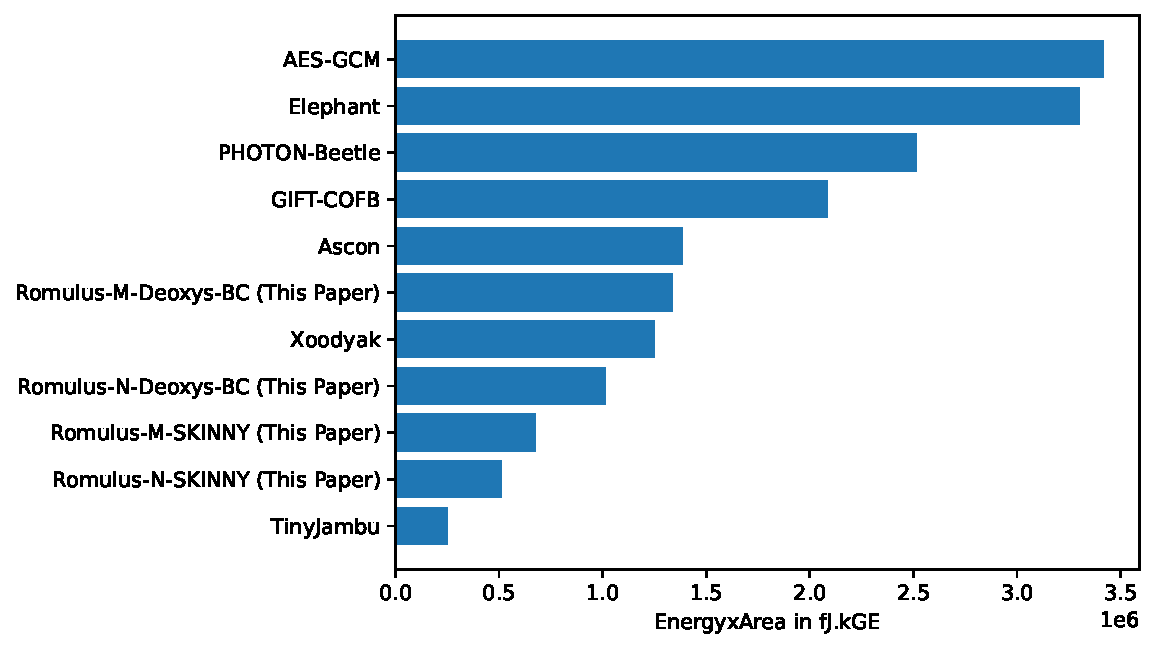
\includegraphics[width=0.49\textwidth]{figures/withM_energy_area64_bar_65.pdf}
  \caption{Energy$\times$Area product for 64 bytes of $A$ and $M$ for various AEAD schemes.}\label{fig:energy_area_64}
\end{figure}

\begin{figure}[!h]
  \centering
  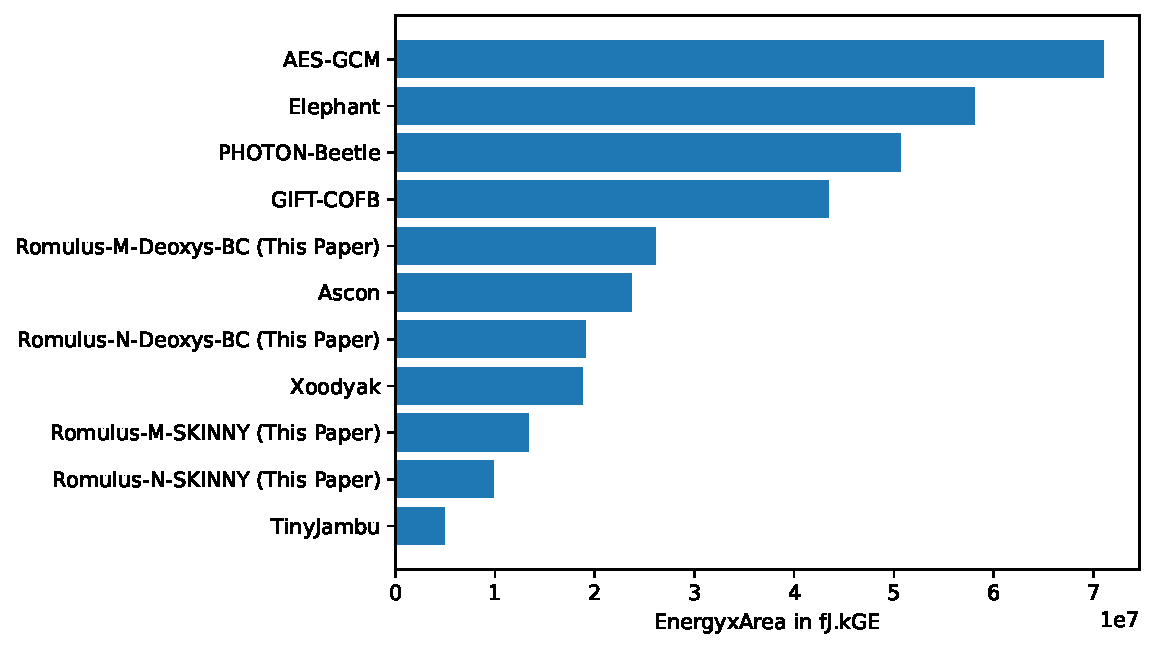
\includegraphics[width=0.49\textwidth]{figures/withM_energy_area1536_bar_65.pdf}
  \caption{Energy$\times$Area product for 1536 bytes of $A$ and $M$ blocks for various AEAD schemes.}\label{fig:energy_area_1536}
\end{figure}


\section{Future Work}

The proposed accelerator can be configured for multiple shares of the SRF and the KRF. However, the corresponding masked circuits of the TBC need to be designed and tested. We leave this as part of a different ongoing research project. Additionally, we will explore integrating other TBC-based primitives, such as public hashing, in the proposed accelerator.



\bibliographystyle{IEEEtran}
\bibliography{ispled}


\end{document}
